\documentclass[a4paper]{article}
\usepackage[spanish]{babel}
\selectlanguage{spanish}
\usepackage[utf8]{inputenc}
\usepackage[T1]{fontenc}

\usepackage[a4paper,top=3cm,bottom=1.25cm,left=1.75cm,right=1.75cm,marginparwidth=1.75cm]{geometry}

\usepackage{amsmath, amsthm, amsfonts}
\usepackage{graphicx}
\usepackage[colorinlistoftodos]{todonotes}
\usepackage[colorlinks=true, allcolors=blue]{hyperref}

\usepackage{listings}
\usepackage{xcolor}

\definecolor{codegreen}{rgb}{0,0.6,0}
\definecolor{codegray}{rgb}{0.5,0.5,0.5}
\definecolor{codepurple}{rgb}{0.58,0,0.82}
\definecolor{backcolour}{rgb}{0.95,0.95,0.92}

\lstdefinestyle{mystyle}{
    backgroundcolor=\color{backcolour},   
    commentstyle=\color{codegreen},
    keywordstyle=\color{magenta},
    numberstyle=\tiny\color{codegray},
    stringstyle=\color{codepurple},
    basicstyle=\ttfamily\footnotesize,
    breakatwhitespace=false,         
    breaklines=true,                 
    captionpos=b,                    
    keepspaces=true,                 
    numbers=left,                    
    numbersep=5pt,                  
    showspaces=false,                
    showstringspaces=false,
    showtabs=false,                  
    tabsize=2
}
\graphicspath{ {screenshots/} }
\lstset{style=mystyle}

\title{Born2beRoot}
\author{Miguel Mazuelo Álvarez\\
  \small 42 Madrid\\
  \small mmazuelo@student.42madrid.com\\
  \date{}
}

\begin{document}
\maketitle

\begin{abstract}
Este documento es un ejercicio de administración de sistemas.
\end{abstract}

\section{Parte obligatoria}
\subsection{Selecci\'on del sistema operativo}
He seleccionado CentOS principalmente para entender su complejidad, así como para entender mejor sistemas operativos de Red Hat, como por otro lado ponerme a prueba con \textit{bash}

\subsection{Instalaci\'on}
\begin{itemize}
\item Le he facilitado 30.8GB para hacer la parte bonus.
\item 2GB de RAM es suficiente para poder correr.
\item Se instala la versión CentOS Linux 7
\end{itemize}
La version CentOS Linux 8, fue destruida el \date{31-12-2021} ya que se quieren centrar en CentOS Stream 8 (esta versión carece de instalación mínima y solo existe en versión escritorio).\footnote{https://www.centos.org/}

\subsubsection{LVM}

\subsection{Configurando CentOS}
\subsubsection{Instalando dnf}
 \textbf{dnf} es un gestor de paquetes para distribuciones basadas en RPM\footnote{Red Hat Package Manager}, siendo una versión mejorada de \textbf{yum}.\\
Primeramente comprobamos si tenemos instalada alguna version de \textbf{dnf}. Por lo tanto introducimos:
\begin{lstlisting}[language=Bash]
dnf --version
\end{lstlisting}
Para instalarlo nos apoyamos con \textbf{yum}. Al meter como argumento \textbf{-y} en la instalación estamos aceptamos todo aquello que nos pregunte miestras se instala el paquete.
\begin{lstlisting}[language=Bash]
yum install dnf -y
\end{lstlisting}

\subsubsection{SELinux}
\paragraph{AppArmor}

\pagebreak

\subsubsection{UFW}
Primeramente habilitamos la paquetería adicional de EPEL\footnote{EPEL (Extra Packages for Enterprise Linux) se trata de un conjunto de paquetes adicionales que normalmente no estarían disponibles en Enterprise Linux.} ya que \textbf{ufw} no está disponible en el repositorio de CentOS
\begin{lstlisting}[language=Bash]
dnf install epel-release -y
\end{lstlisting}
Instalamos, ahora sí, \textbf{ufw} y lo habilitamos.
\begin{lstlisting}[language=Bash]
dnf install ufw -y
ufw enable
\end{lstlisting}
Comprobamos si está activo.
\begin{lstlisting}[language=Bash]
ufw status verbose
\end{lstlisting}
Habilitamos para la entrada y salida de datos, y nuestro puerto.
\begin{lstlisting}[language=Bash]
ufw default allow incoming
ufw default allow outgoing
ufw allow 4242
\end{lstlisting}
Eliminamos los otros canales dejando solo al puerto 4242.
\begin{lstlisting}[language=Bash]
ufw status numbered
ufw delete 1
...
\end{lstlisting}
\begin{figure}[h]
\centering
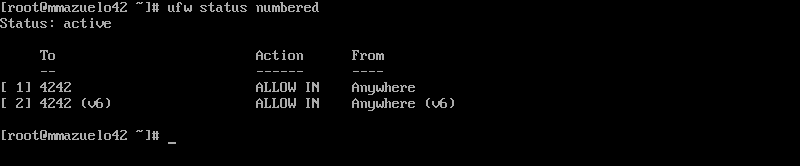
\includegraphics[scale=0.5]{15_CentOS42_ufw_port4242}
\end{figure}

\noindent Habilitamos \textbf{ufw} para que se habilite en el arranque.
\begin{lstlisting}[language=Bash]
systemctl enable ufw
\end{lstlisting}
Reinciamos para que se apliquen los cambios
\begin{lstlisting}[language=Bash]
systemctl restart ufw
\end{lstlisting}
\paragraph{firewalld}
Es el firewall por defecto de CentOS
\\
Comprobamos si lo tenemos activo:
\begin{lstlisting}[language=Bash]
systemctl status firewalld
--------------------------------------
firewall-cmd --state
\end{lstlisting}
En caso que lo esté, lo desactivamos...
\begin{lstlisting}[language=Bash]
systemctl stop firewalld
systemctl disable firewalld
systemctl status firewalld
\end{lstlisting}

\pagebreak

%\subsubsection{ssh}
%dnf install openssh -y
%systemctl start sshd
%systemctl enable sshd
%systemctl status sshd

%vi /etc/ssh/sshd_config
%	Port 22 -> 4242
%	PermitRootLogin no
%	PubkeyAuthentication yes


%dnf whatprovides semanage
%dnf install policycoreutils-python -y
%semanage -h
%semanage port -l | grep ssh
%semanage port -a -t ssh_port_t -p tcp 4242
%systemctl restart sshd
%semanage port -l | grep ssh
5274 3400 1229 2155 04/24 631

\subsubsection{sudo}

\section{Bonus}


\end{document}